\begin{center}
\Large\textbf{\textsf{ÉTUDE DU SISMOMÈTRE SEIS}}
\normalsize
\end{center}
\section{Présentation}
Après des années de recherche et de développement puis un voyage de 485 millions de kilomètres, la sonde InSight (Interior Exploration using Seismic Investigations, Geodesy and Heat Transport) s'est posée sur Mars le 26 novembre 2018. Elle est le premier observatoire géophysique martien, dont l'objectif est d'étudier la structure interne de Mars et de comprendre la formation et l'évolution des planètes rocheuses du Système solaire. En mesurant la façon dont les ondes sismiques, provoquées par des séismes martiens ou des impacts de météorites, se propagent à l'intérieur de Mars, les géophysiciens vont pouvoir répondre avec précision à cet objectif.


\begin{figure}[!h]
\centering
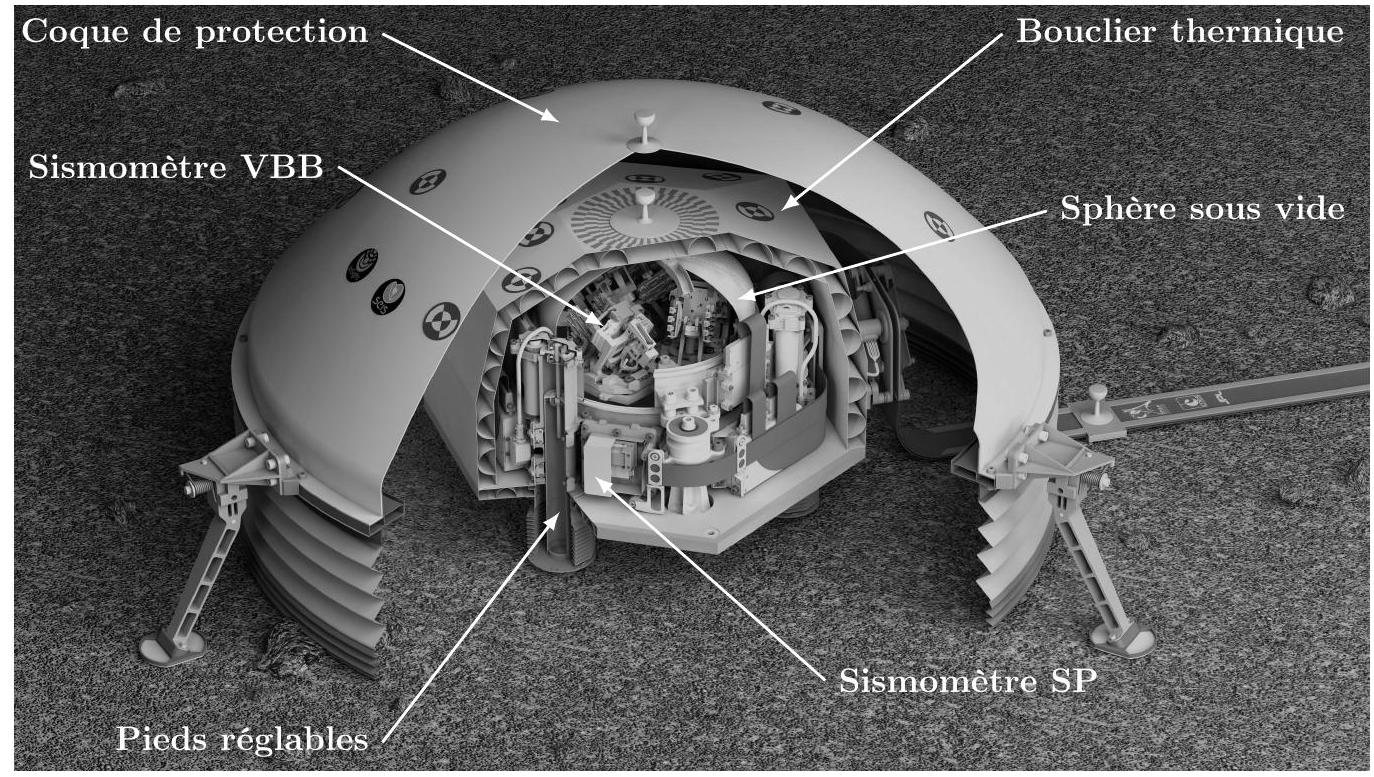
\includegraphics[width=.6\textwidth]{2024_04_26_3285cfc264024262add0g-02}
\caption{\label{ccmp2023_fig_01}Écorché de SEIS et ses différents niveaux de protection}
%FigURE 1 - Écorché de SEIS et ses différents niveaux de protection}
\end{figure}




Le sismomètre SEIS (Seismic Experiment for Interior Structures), déployé à la surface de Mars, est protégé des variations de la température et du vent à l'aide d'un bouclier thermique et d'une coque de protection. SEIS comporte deux sismomètres indépendants, le VBB (Very Broad Band) et le SP (Short Periods), montés sur une structure commune pouvant être réglée à l'horizontale grâce à des pieds de longueur variable.

\begin{itemize}
  \item Le sismomètre VBB comporte trois systèmes identiques, composés chacun d'un pendule et d'un bâti, inclinés différemment par rapport au sol. Ils sont fixés dans une sphère en titane sous vide, et sensibles à une large bande de fréquence d'ondes sismiques, entre \SI{0,01}{Hz} et $0,5 \si{Hz}$.
  \item Le sismomètre SP est adapté aux ondes sismiques de plus hautes fréquences, entre 0,1 et $50 \si{Hz}$.
\end{itemize}

\begin{figure}[!h]
\centering
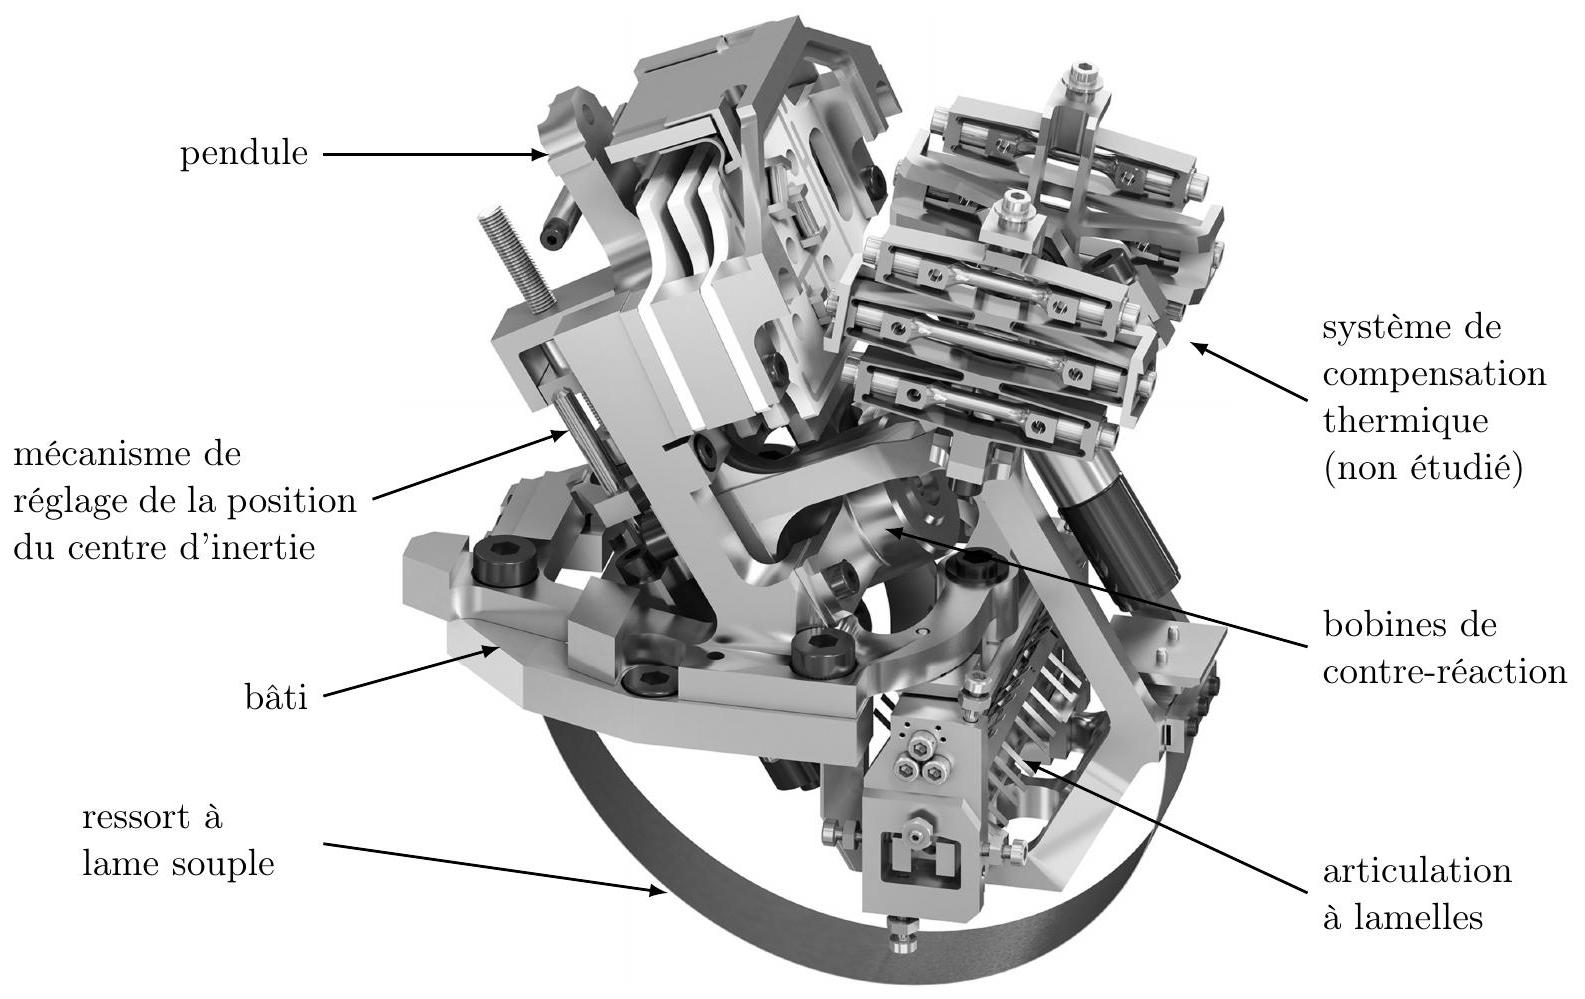
\includegraphics[width=.7\textwidth]{2024_04_26_3285cfc264024262add0g-03}
\caption{\label{ccmp2023_fig_02} Vue 3D d'un des trois systèmes du VBB}
% Figure 2 - Vue 3D d'un des trois systèmes du VBB
\end{figure}



Dans ce sujet, on s'attache à valider certaines étapes clés de la conception et du réglage d'un des trois systèmes du sismomètre VBB. Cette dernière étape ayant eu lieu sur Terre, il a fallu contourner les difficultés liées aux différences de gravité et de température entre la Terre et Mars.

Une vue détaillée d'un des systèmes du VBB est fournie en figure \ref{ccmp2023_fig_02} et le détail des différents éléments qui le constituent est fourni en Annexe 1.
